\section{\S 3.3 酸碱滴定\texorpdfstring{（又称中和滴定）}{}}\label{sect:酸碱滴定}

    \subsection{中和滴定的原理}\label{subsec:中和滴定的原理}

        \begin{xmp}
            [中和滴定计算例题]
            {}
            []
            []
            在 \SI{20.00}{mL} 盐酸中逐滴滴入 \SI{0.1116}{\mole\per\litre} 的氢氧化钠溶液，当滴至 \SI{21.90}{mL} 时，恰好完全反应。计算该盐酸的浓度。

            \vspace{0.5\baselineskip}
            \begin{minipage}{0.55\textwidth}

                \cemh{HCl + NaOH \xleq{} NaCl + H2O}
            
                完全反应时：\(n(\cemh{HCl} = n(\cemh{NaOH}))\)

                \(\therefore c(\cemh{HCl})\cdot V(\cemh{HCl}) = c(\cemh{NaOH}) \cdot V(\cemh{NaOH})\)

                \(\therefore c(\cemh{HCl}) = c(\cemh{NaOH})\cdot\frac{V(\cemh{NaOH})}{V(\cemh{HCl})}\)
            \end{minipage}
            \hfil
            \begin{minipage}{0.35\textwidth}
                \hfil\textcolor{red}{\SI{0.1222}{\mole\per\litre}}
                \newline
                \newline
                \textcolor{red}{盐酸是一元酸、氢氧化钠是一元碱，如果酸、碱不是一元的，则应注意酸碱反应的比例。}
            \end{minipage}
        \end{xmp}

        \textcolor{blue}{计算通式：}\(c_\text{酸}\cdot V_\text{酸}\cdot N_\text{酸}=c_\text{碱}\cdot V_\text{碱}\cdot N_\text{碱}\)

        \(c\)—浓度，\(V\)—体积，\(N\)—酸碱元数

        中和滴定——用已知浓度的酸（或碱）溶液来测定未知浓度的碱（或酸）溶液的方法

        标准液：已知浓度的溶液

        待测液：未知浓度的溶液

        滴定终点：酸碱恰好完全反应

        \noindent\textcolor{red}{中和滴定的关键之一——正确判断滴定终点}

        \textcolor{red}{如何准确判断中和反应是否恰好完全反应了呢？}

        \textcolor{red}{盐酸与氢氧化钠中和是否有反应现象？}

        \textcolor{red}{如何创造出反应现象？}

        \textcolor{blue}{利用酸碱指示剂的颜色变化}

        \noindent\textcolor{red}{中和滴定的关键之二——如何精确地测定酸、碱的体积}

        \vspace{-0.5\baselineskip}
        \[
            \underset{\text{待测}}{\underset{\uparrow}{c(\cemh{HCl})}} = \underset{\text{已知}}{\underset{\uparrow}{c(\cemh{NaOH})}}\cdot\left.\frac{V(\cemh{NaOH})}{V(\cemh{HCl})}\right\}\makebox{一个事先量取，另一个滴加测量}
        \]

        \textcolor{blue}{需要一个特殊的仪器——既能滴加液体，又能测量液体体积}

    \subsection{实验仪器}\label{subsec:实验仪器}

        \subsubsection{滴定管}\label{subsubsec:滴定管}
                \begin{enumerate}
                \item 零刻度在上，最大刻度在下
                    
                \( \text{液体体积} = \text{末读数} - \text{初读数} \)
                
                \textcolor{blue}{有\SI{25}{\milli\litre}、\SI{50}{\milli\litre}两种规格}
                \item 最小刻度\SI{0.1}{\milli\litre}，估读至\SI{0.01}{\milli\litre}
                
                数据记录至小数点后第二位\textcolor{red}{（很重要！）}
                \item 读数方法：蓝线的粗细交界点\textcolor{red}{（平视！）}
                \item 检验：活塞处是否漏水
                \item 洗涤：分为用自来水洗、用蒸馏水润洗、用所盛溶液润洗三步
            \end{enumerate}
        
        \subsubsection{锥形瓶\texorpdfstring{\textcolor{blue}{——反应场所}}{}}\label{subsubsec:锥形瓶}
            洗涤：分为用自来水洗、用蒸馏水润洗二步

    \subsection{滴定过程}\label{subsec:滴定过程}

        \begin{enumerate}
            \item 装液，赶气泡
            \item 读出待测液（或标准液）初读数，放一定量至锥形瓶中，读末读数
            \item 加入指示剂\numrange{2}{3}滴\textcolor{red}{（千万别忘记）}
            \item 读另一初读数，用标准液（或待测液）滴定\textcolor{red}{（先快后慢，最后一滴滴地加）}
            \item 滴到加入最后半滴时，指示剂变色，\uline{并保持半分钟不复原}，停止滴定，读末读数
            \item 洗净锥形瓶，装液，重复滴定\numrange{2}{3}次
        \end{enumerate}

        \subsubsection{操作姿势}\label{subsubsec:滴定操作姿势}

        \begin{enumerate}
            \item 一手拿锥形瓶，并在滴定过程中不断摇晃
            \item 一手控制滴定管活塞
            \item 眼睛始终注视锥形瓶，观察溶液颜色变化
        \end{enumerate}

        \subsubsection{中学阶段常用的指示剂}\label{subsubsec:滴定中学阶段常用的指示剂}

        \begingroup
        \setlength{\fboxsep}{0pt}
        % \small
        \newcommand{\boxstrut}{\rule[-0.2em]{0pt}{1.2em}}
        \begin{center}
        \begin{tabular}{lll}
            甲基橙 &\small 1\colorbox{red}{\makebox[4.2em]{\boxstrut 红色}}\colorbox{orange}{\makebox[2.6em]{\boxstrut 橙色}}\colorbox{yellow}{\makebox[15.2em]{\boxstrut 黄色}}12 & --3.1--4.4-- \\
            甲基红 &\small 1\colorbox{red}{\makebox[6.8em]{\boxstrut 红色}}\colorbox{orange}{\makebox[3.6em]{\boxstrut 橙色}}\colorbox{yellow}{\makebox[11.6em]{\boxstrut 黄色}}12 & --4.4--6.2-- \\
            石蕊   &\small 1\colorbox{red}{\makebox[7em]{\boxstrut 红色}}\colorbox{violet!85!white}{\makebox[7.6em]{\boxstrut \color{white}紫色}}\colorbox{blue}{\makebox[7.4em]{\boxstrut \color{white}蓝色}}12 & --4.5--8.3-- \\
            酚酞   &\small 1\colorbox{gray!25!white}{\makebox[14em]{\boxstrut 无色}}\colorbox{red!50!white}{\makebox[4em]{\boxstrut 粉红色}}\colorbox{red}{\makebox[4em]{\boxstrut 红色}}12 & --8.0--10.0-- \\
        \end{tabular}
        \end{center}
        \endgroup
        \textcolor{red}{指示剂选择要求：颜色变化敏锐、明显}

        \subsubsection{酸碱中和滴定过程中的 pH 变化}\label{subsubsec:酸碱中和滴定过程中的pH变化}

        \noindent\textbf{【计算填表】：\SI{0.1}{\mol\per\litre} \cemh{NaOH} 滴定 20.00 mL \SI{0.1}{\mol\per\litre} 盐酸（碱滴酸）}
        \begin{center}
        \small
        \begin{tabular}{|c|c|c|c|c|c|}
            \hline
            加入 \cemh{NaOH}  & 剩余盐酸 & 过量 \cemh{NaOH}  & 溶液总 & \cemh{[H+]} & pH \\
            的体积(\si{\milli\litre}) & (\si{\milli\litre}) &  的体积(\si{\milli\litre}) &体积(\si{\milli\litre}) & (\si{\mol\per\litre}) & \\
            \hline
            \num{0.00}  & \num{20.00} & --    & \num{20.00} & \num{0.1}           & \num{1.00} \\ 
            \num{10.00} & \num{10.00} & --    & \num{30.00} & \num{0.0333}        & \num{1.48} \\ 
            \num{18.00} & \num{2.00}  & --    & \num{38.00} & \num{5.263E-3}     & \num{2.28} \\ 
            \num{19.80} & \num{0.20}  & --    & \num{39.80} & \num{5.025E-4}     & \num{3.30} \\ 
            \num{19.98} & \num{0.02}  & --    & \num{39.98} & \num{5.003E-5}     & \num{4.30} \\ 
            \num{20.00} & \num{0}     & --    & \num{40.00} & \num{1E-7}     & \num{7.00} \\ 
            \num{20.02} & --          & \num{0.02} & \num{40.02} & \num{2.001E-10} & \num{9.70} \\ 
            \num{20.20} & --          & \num{0.20} & \num{40.20} & \num{2.01E-11}  & \num{10.70} \\ 
            \num{22.00} & --          & \num{2.00} & \num{42.00} & \num{2.1E-12}   & \num{11.68} \\ 
            \num{30.00} & --          & \num{10.00}& \num{50.00} & \num{5E-13}     & \num{12.30} \\ 
            \num{40.00} & --          & \num{20.00}& \num{60.00} & \num{3E-13}     & \num{12.52} \\
            \hline
        \end{tabular}
        \end{center}

        以溶液的 pH 变化为纵坐标，以消耗的 \cemh{NaOH} 体积为横坐标，画出滴定过程中溶液 pH 变化的曲线图

        \begin{figure}[h!]
            \centering
            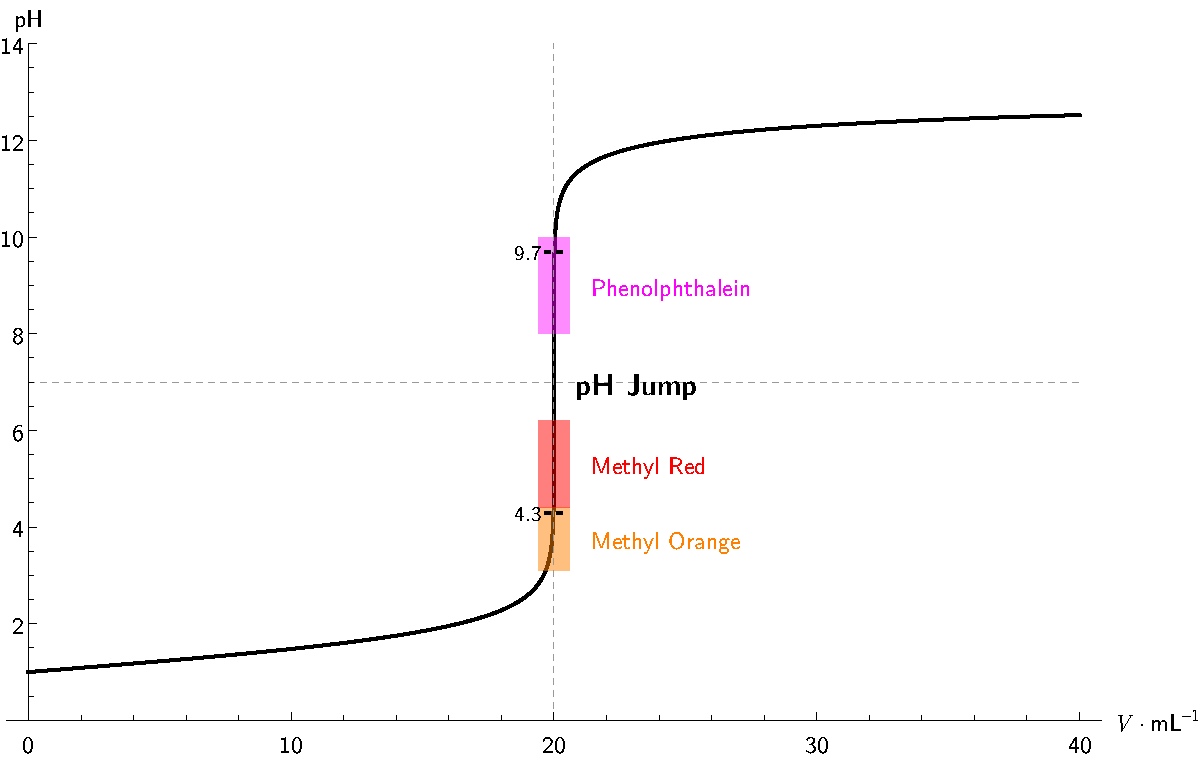
\includegraphics[width=\textwidth]{chapters/titration_indicators_2501.pdf}
            \caption{\SI{0.1}{\mol\per\litre} \cemh{NaOH} 滴定 20.00 mL \SI{0.1}{\mol\per\litre} 盐酸的 pH 变化}
            \label{fig:titration_indicators_2501}
        \end{figure}

        \textcolor{red}{\numrange{4.3}{9.7}，只需要\SI{0.04}{\milli\litre}，即\SI{1}{\text{滴}}溶液（\(\SI{1}{\milli\litre}=\SI{25}{\text{滴}}\)）}

        \textcolor{blue}{指示剂的变色范围要在滴定突跃范围内}

        \textcolor{red}{\(\therefore\)即使过量或不足量，\(\text{误差} \leq \SI{0.02}{\milli\litre}\)（半滴），相对误差 \(\leq \SI{1}{\text{\textperthousand}}\)}

    \subsection{指示剂选择与滴定过程中的颜色变化}\label{subsec:指示剂选择与滴定过程中的颜色变化}

        \begin{enumerate}
            \item 常用酚酞与甲基橙（或甲基红）\footnote{以下分析中甲基橙均可用甲基红替代}；石蕊不宜选用（颜色变化不明显）
            \item 强酸、强碱滴定时，均可选用
            
            \begin{center}
            \begin{tabular}{@{}lcc@{}}
            \toprule
            & 强酸滴强碱 & 强碱滴强酸 \\
            \midrule
            甲基橙 & 黄\(\to\)橙 & 橙\(\to\)红 \\
            酚酞   & 红\(\to\)粉红 & 无\(\to\)粉红 \\
            \bottomrule
            \end{tabular}
            \end{center}
            
            一般：酸滴碱用甲基橙，碱滴酸用酚酞。

            \textcolor{red}{原则：浅色\(\to\)深色}

            \item 强碱滴弱酸
            
            比如：NaOH 溶液滴定醋酸

            \textcolor{red}{原则：反应后盐溶液的酸碱性。选择变色范围接近的指示剂}

            \( \therefore \) 用酚酞

            \item 强酸滴弱碱
            
            用甲基橙或甲基红

        \end{enumerate}

        \begin{figure}[h!]
            \centering
            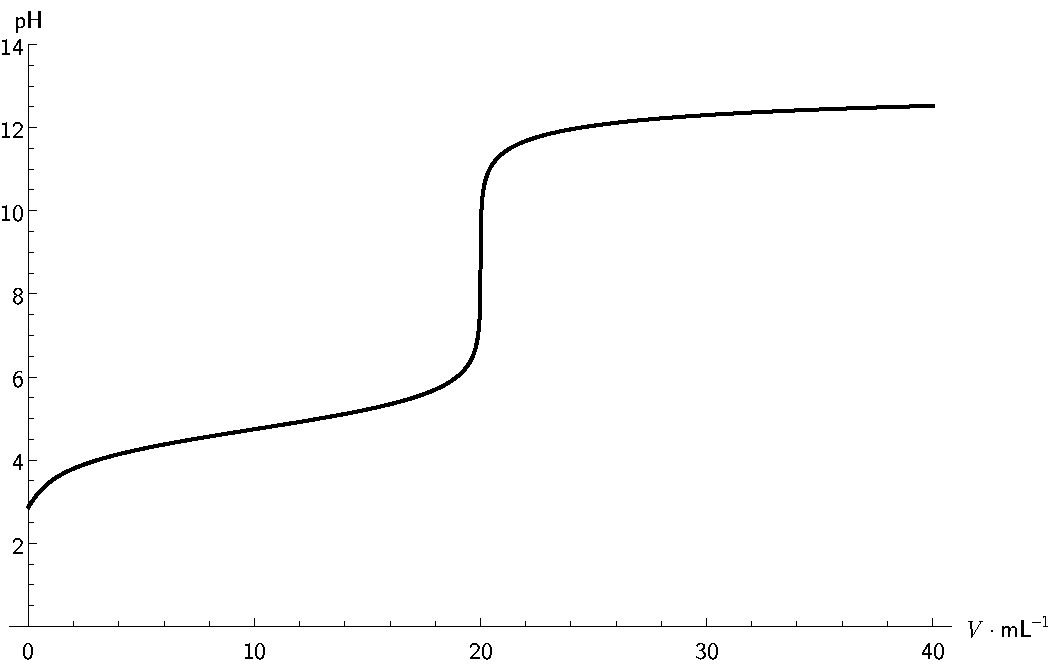
\includegraphics[width=\textwidth]{chapters/titration_acetic_2501.pdf}
            \caption{\SI{0.1}{\mol\per\litre} \cemh{NaOH} 滴定 20.00 mL \SI{0.1}{\mol\per\litre} 醋酸的 pH 变化}
            突跃范围：pH \numrange{7.7}{9.7}
            \label{fig:titration_acetic_2501}
        \end{figure}

    \subsection{误差分析}\label{subsec:误差分析}

        已知：用标准盐酸滴定待测氢氧化钠溶液。下列因素对该实验测定结果是否有影响？如有影响测定结果偏大还是偏小？

        \begin{enumerate}
            \item 滴定时，滴在锥形瓶外一滴盐酸\dotfill\textcolor{blue}{〔偏大〕}
            \item 锥形瓶水洗后直接装入待测 NaOH 溶液\dotfill\textcolor{blue}{〔不变〕}
            \item 锥形瓶水洗后用待测 NaOH 溶液润洗\dotfill\textcolor{blue}{〔偏大〕}
            \item 滴定管水洗后没用待测 NaOH 溶液润洗\dotfill\textcolor{blue}{〔偏小〕}
            \item 滴定管水洗后没有用标准盐酸润洗\dotfill\textcolor{blue}{〔偏大〕}
            \item （碱）开始读数时正确，结束时读数俯视\dotfill\textcolor{blue}{〔偏大〕}
            \item （酸）开始读数时仰视，结束时读数正确\dotfill\textcolor{blue}{〔偏小〕}
            \item （酸）滴定开始读数时未赶走气泡，结束时气泡消失\dotfill\textcolor{blue}{〔偏大〕}
            \item （酸）滴定开始读数时未赶走气泡，结束时仍有气泡\dotfill\textcolor{blue}{〔未知〕}
        \end{enumerate}

    \subsection{典型案例分析}\label{subsec:滴定典型案例分析}

        \begin{xmp}
            [测定小苏打样品的纯度]
            {测定小苏打样品的纯度（杂质为氯化钠）}
            []
            []
            \begin{itemize}
                \item 反应原理：\cemh{NaHCO3 + HCl \xleq{} NaCl + H2O + CO2 ^}
                \item 需要测定的量：样品质量、滴定消耗盐酸体积
                \item 实验步骤：
                \vspace{-0.5\baselineskip}
                \[
                    \overset{\makebox{样品}}{\overset{\makebox{\(\downarrow\)}}{\underset{\makebox{\(m\)\,\si{\gram}}}{\text{称量}}}}
                    \longrightarrow
                    \overset{\makebox{指示剂}}{\overset{\makebox{\(\downarrow\)}}{\underset{}{\text{滴加}}}}
                    \longrightarrow
                    \overset{\makebox[4em][l]{标准盐酸\(c\)\,\si{\mole\per\litre}}}{\overset{\makebox{\(\downarrow\)}}{\underset{\makebox{\(V\)\,\si{\milli\litre}}}{\text{滴定}}}}
                    \phantom{\makebox{\si{\mole\per\litre}}}
                \]

                \item 指示剂应选用：\textcolor{red}{甲基橙或甲基红}
                \item \textcolor{blue}{按\(c=\SI{0.1}{\mole\per\litre}\)、\(V=\SI{10}{\milli\litre}\)}
                
                \textcolor{blue}{计算每次大约称多少克样品：}\textcolor{red}{\SI{0.084}{\gram}}
                
                \textcolor{red}{怎么解决称量太小，称量的相对误差大？}

                \item 实验步骤：\hfil\textcolor{blue}{\( \therefore \) 滴定法测定时，常需要配合使用容量瓶}
                \[
                    \overset{\makebox{样品}}{\overset{\makebox{\(\downarrow\)}}{\underset{\makebox{\(m\)\,\si{\gram}}}{\text{称量}}}}
                    \longrightarrow
                    \overset{\makebox{蒸馏水}}{\overset{\makebox{\(\downarrow\)}}{\underset{\makebox{\(a\)\,\si{\milli\litre}}}{\text{配溶液}}}}
                    \longrightarrow
                    \underset{\makebox{\(b\)\,\si{\milli\litre}}}{\text{量取}}
                    \longrightarrow
                    \overset{\makebox{指示剂}}{\overset{\makebox{\(\downarrow\)}}{\underset{}{\text{滴加}}}}
                    \longrightarrow
                    \overset{\makebox[4em][l]{标准盐酸\(c\)\,\si{\mole\per\litre}}}{\overset{\makebox{\(\downarrow\)}}{\underset{\makebox{\(V\)\,\si{\milli\litre}}}{\text{滴定}}}}
                    \phantom{\makebox{\si{\mole\per\litre}}}
                \]

                \item 计算式：
                \vspace{-1.5\baselineskip}

                \[
                    \cemh{NaHCO3}\si{\percent}=\frac{\frac{c\cdot V}{1000} \times \frac{a}{b} \times 84}{m} \times \SI{100}{\percent}
                \]
            \end{itemize}
        \end{xmp}
    
        \begin{xmp}
            [返滴定法]
            {测定鸡蛋壳中的 \cemh{CaCO3} 含量（返滴定法）}
            []
            []
            \textcolor{red}{无法直接滴定，如何用滴定法测定？能否转换成酸碱滴定？}
            \begin{itemize}
                \item 反应原理：\cemh{CaCO3 + 2HCl \xleq{} CaCl2 + H2O + CO2 ^}
                
                \phantom{反应原理：}\cemh{HCl + NaOH \xleq{} NaCl + H2O}
                \item 实验步骤：
                \vspace{-0.5\baselineskip}
                \[
                    \text{鸡蛋壳}
                    \longrightarrow
                    \text{粉碎}
                    \longrightarrow
                    \text{称量}
                    \longrightarrow
                    \overset{\makebox{足量盐酸}}{\overset{\makebox{\(\downarrow\)}}{\underset{}{\text{酸溶}}}}
                    \longrightarrow
                    \overset{\makebox{蒸馏水}}{\overset{\makebox{\(\downarrow\)}}{\underset{\makebox{\(a\)\,\si{\milli\litre}}}{\text{配溶液}}}}
                    \longrightarrow
                \]
                \[
                    \longrightarrow
                    \underset{\makebox{\(b\)\,\si{\milli\litre}}}{\text{量取}}
                    \longrightarrow
                    \overset{\makebox{指示剂}}{\overset{\makebox{\(\downarrow\)}}{\underset{}{\text{滴加}}}}
                    \longrightarrow
                    \overset{\makebox{标准 \cemh{NaOH} 溶液}}{\overset{\makebox{\(\downarrow\)}}{\underset{}{\text{滴定}}}}
                \]

                \item 计算需要的物理量：鸡蛋壳的质量、盐酸的浓度和体积、\cemh{NaOH} 溶液的浓度和体积
            \end{itemize}
        \end{xmp}

    \subsection[氧化还原滴定]{氧化还原滴定——利用氧化还原反应的滴定测定法}\label{subsec:拓展：氧化还原滴定}

        \subsubsection{高锰酸钾法}\label{subsubsec:高锰酸钾法氧化还原滴定}

            \textcolor{red}{需酸化，通常用 \cemh{H2SO4}，不使用 \cemh{HCl} 或 \cemh{HNO3}}

            \vspace{-0.5\baselineskip}
            \[\cemh{MnO4- + 5 e- + 8H+ \xleq{} Mn^2+ + 4H2O}\]

            \textcolor{blue}{优点：氧化能力强、可测定物质多，一般不需要另加指示剂}

            \begin{enumerate}
                \item 直接滴定
                
                测定还原性物质，如：\cemh{Fe^2+}、\cemh{H2O2}、\cemh{H2C2O4}、\cemh{Sn^2+} 等

                滴定终点判断：当滴入最后半滴后，溶液显浅紫红色，\uline{并保持半分钟不复原}

                \item 返滴定
                
                测定氧化性物质，如：\cemh{MnO2}、\cemh{Pb2O4}、\cemh{K2Cr2O7}、\cemh{KClO3} 等

                \begin{xmp}
                    [软锰矿中 MnO2 的含量测定]
                    {软锰矿中 \cemh{MnO2} 的含量测定}
                    []
                    []
                    在 \cemh{H2SO4} 存在下，加入一定量且过量的 \cemh{Na2C2O4}，加热充分反应后，用标准 \cemh{KMnO4} 溶液滴定过量的 \cemh{C2O4^2-}。
                \end{xmp}

                \item 间接滴定
                
                \begin{xmp}
                    [Ca2+含量测定]
                    {\cemh{Ca^2+} 含量测定}
                    []
                    []
                    首先用 \cemh{C2O4^2-} 将 \cemh{Ca^2+} 沉淀为 \cemh{CaC2O4}，过滤，再用稀 \cemh{H2SO4} 将 \cemh{CaC2O4} 沉淀溶解，然后用标准 \cemh{KMnO4} 溶液滴定 \cemh{H2C2O4}，从而间接求得 \cemh{Ca^2+} 含量。
                \end{xmp}

            \end{enumerate}
            
        \subsubsection{碘量法}\label{subsubsec:碘量法氧化还原滴定}
        
            \textcolor{blue}{用淀粉溶液作指示剂}

            \begin{enumerate}
                \item 直接碘量法\textcolor{red}{（碘标准溶液）}
                
                测定较强的还原剂，如：\cemh{S^2-}、\cemh{SO3^2-}、\cemh{Sn^2+}、\cemh{V_C} 等

                例如 \cemh{V_C} 与 \cemh{I2} 反应： \cemh{C6H8O6 + I2 -> C6H6O6 + 2HI}

                滴定终点判断：当滴入最后半滴后，溶液显蓝色，\uline{并保持半分钟不复原}

                \item 间接碘量法\textcolor{red}{（\cemh{Na2S2O3} 标准溶液）}
                
                测定氧化性物质，如 \cemh{H2O2}、\cemh{Cu^2+}、\cemh{KIO3}、\cemh{NaClO} 等

                先与过量的 \cemh{KI} 反应生成 \cemh{I2}，用 \cemh{Na2S2O3} 标准溶液滴定生成的 \cemh{I2}，从而计算得到氧化性物质的量。\cemh{2S2O3^2- + I2 \xleq{} S4O6^2- + 2I-}

                滴定终点判断：当滴入最后半滴后，溶液蓝色褪去，\uline{并保持半分钟不复原}

                注意事项：
                \begin{enumerate}
                    \item 加入过量的 \cemh{KI}，形成 \cemh{I3-}（\cemh{I- + I2 \xleq{} I3-}），降低 \cemh{I2} 的挥发性
                    \item 由于 \cemh{I-} 易被 \cemh{O2} 氧化，滴定时不宜剧烈摇动锥形瓶
                \end{enumerate}

            \end{enumerate}
